\documentclass[10pt,a4paper]{article}
\usepackage[utf8]{inputenc}
\usepackage[english]{babel}
\usepackage[T1]{fontenc}
\usepackage{amsmath}
\usepackage{amsfonts}
\usepackage{amssymb}
\usepackage{subcaption}
\usepackage{makeidx}
\usepackage{graphicx}
\usepackage{fourier}
\usepackage{listings}
\usepackage{color}
\usepackage{hyperref}
\usepackage[left=2cm,right=2cm,top=2cm,bottom=2cm]{geometry}
\author{Tommy Müller, Marcus Dittrich, Vincent Noculak}
\title{Rastertunnelmikroskopie}

\lstset{language=C++,
	keywordstyle=\bfseries\color{blue},
	commentstyle=\itshape\color{red},
	stringstyle=\color{green},
	identifierstyle=\bfseries,
	frame=single}
\begin{document}

\maketitle
\newpage
\tableofcontents
\newpage

	\section{ Theoretische Vorbereitung}
	
	Das Rastertunnelmikroskop ist eine Vorrichtung, mit der sich Festkörperstrukturen in atomarer Größenordnung auflösen und graphisch darstellen lassen. Der Versuchsaufbau besteht prinzipiell aus einer, wenn möglich, einatomigen Spitze, welche sich mittels eines piezoelektrischen Elements über die Probenoberfläche bewegt. Der Messkopf wird dabei der Probe bis auf wenige $\AA$ angenähert, bis die Überlagerung der Wellenfunktionen von Probe und Spitze es ermöglicht, dass Elektronen die Potentialbarriere zwischen beiden Materialien "durchtunneln". Der dabei messbare Tunnelstrom gibt Aufschlüsse über die lokale Zustandsdichte der Probe, aus der man Rückschlüsse auf dessen Struktur an der Oberfläche ziehen kann. \\ \\Das "Durchtunneln" einer endlichen Potenzialbarriere, welche höher als die kinetische Energie des "durchtunnelnden" Teilchens ist, kann nur mit Hilfe der Quantenmechanik erklärt werden. In der quantenmechanischen Betrachtungsweise wird das Teilchen als Wellenfunktion in der Schrödingergleichung angenommen und besitzt dadurch eine gewisse Wahrscheinlichkeit die Barriere zu durchdringen. Anschaulich lässt sich dies bei dem eindimensionalen Tunnelvorgang durch ein rechteckiges Potential der Breite d und Höhe $\Phi$ darstellen, wie in Figure 1 gezeigt.
	\begin{figure}[h]
		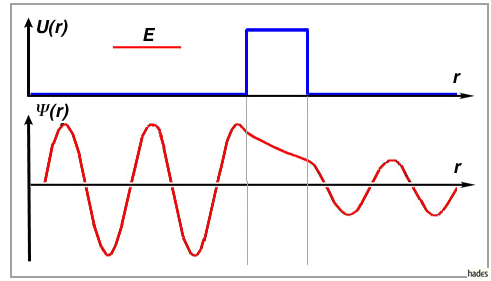
\includegraphics[scale = 0.8]{tunnel.png}
		\centering
		\caption{Abbildung Eindimensionaler Tunneleffekt}
		\label{diagramm_aufspaltung}
	\end{figure}
	Die Wellenfunktion des Teilchens lässt sich in drei Teile (vor ($\Psi_{1}$), in ($\Psi_{2}$) und hinter ($\Psi_{3}$) der Barriere) aufteilen. Eine mögliche Lösung für $\Psi$ sieht wie folgt aus:\\
	$$\Psi_{1}= -\frac{k_{2}}{k_{1}}sin(k_{1}x) + cos(k_{1}x)$$ 
	$$\Psi_{2}= e^{-kx}$$
	$$\Psi_{3}= e^{-k_{2}d}(-\frac{k_{2}}{k_{1}}sin(k_{1}(x-d)) + cos(k_{1}(x-d)))$$
	$$ k_{1} = \frac{1}{\hbar}\sqrt{2mE} $$
	$$k_{2} = \frac{1}{\hbar}\sqrt{2m(E-V_{0})}$$
	\\Die Amplitude der einfallenden Wellenfunktion nimmt im Bereich der Potenzialbarriere exponentiell in Abhängigkeit von der Breite und Höhe der Barriere ab. Somit gilt für das Teilchen hinter dem Potential eine von d abhängige Aufenthaltswahrscheinlichkeit, für welche gilt: $\left \langle \Psi  \right \rangle^{2} > 0$. Daraus folgt, dass einfallende Teilchen eine reale Wahrscheinlichkeit besitzen die Potenzialbarriere zu durchdringen, was zu einem messbaren Tunnelstrom führt. \\ \\Das für die Rastertunnelmikroskopie relevante Potenzialtopf-Modell lässt sich analog zum eben beschriebenen Modell der eckigen Potenzialbarriere skizzieren. Spitze und Probe sind leitende Festkörper, deren Fermi-Niveaus sich durch eine angelegte Spannung zwischen Probe und Spitze zueinander verschieben, wodurch Elektronen in unbesetzte Niveaus der anderen Elektrode gelangen können. Die Höhe des Potentials lässt sich aus der Differenz der Elektronenaustrittsarbeiten von Probe und Spitze ermitteln.
	\begin{figure}[h]
		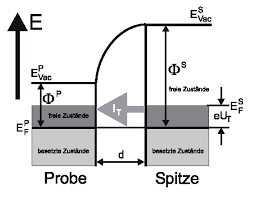
\includegraphics[scale = 1.2]{potentialtopf.png}
		\centering
		\caption{Potentialtopf-Modell zwischen Probe und Spitze}
		\label{diagramm_aufspaltung}
	\end{figure} 
	In Figure 2 wird dieses Konzept schematisch erfasst. Für den sich ergebenden Tunnelstrom lässt sich näherungsweise in Abhängigkeit vom Abstand zwischen Probe / Spitze und der Austrittsarbeit für kleine Probenspannungen folgende Relation festhalten: 
	\begin{equation}
		I_{t} \sim V_{t} * e^{-c*\sqrt{\Phi }*d}
	\end{equation}
	Da man von Austrittsarbeiten in der Größenordnung mehrerer eV ausgehen kann, führt eine Änderung des Abstandes um 1 $\AA$ zu einer Variation des Tunnelstroms um etwa eine Größenordnung. Diese extreme Abstandsabhängigkeit führt dazu, dass man Aussagen im über die elektronische Struktur der Probenoberfläche im atomaren Bereich treffen kann. \\ \\Für die Rastertunnelmikroskopie gibt es im Allgemeinen zwei verschiedene Operationsmodi. Im ersten misst man den Tunnelstrom bei konstantem Abstand zwischen Probe und Spitze, im zweiten misst man den Abstand bei konstant gehaltenem Tunnelstrom. Dies ist der in unserem Versuch verwendete Operationsmodus. \\Um den Abstand zwischen Spitze und Probe so zu variieren, damit der Tunnelstrom konstant bleibt, wird im Allgemeinen ein Regelkreis verwendet. Dieser wirkt der Abweichung einer physikalischen Größe über negative Rückkopplung entgegen, d.h. die Änderung einer bestimmten Größe führt zur proportionalen Änderung einer anderen Größe, welche an das Eingangssignal negativ gekoppelt ist. Vereinfacht gesagt wird der Abstand verringert / vergrößert, je nachdem, ob der gemessene Tunnelstrom  kleiner / größer als der festgelegte Wert ist. Um diese Abstandsänderungen im $\AA$-Bereich vornehmen zu können, wird ein piezoelektrisches Element verwendet. Der diesem Bauteil zugrunde liegende piezoelektrische Effekt besagt, dass eine mechanische Verformung bestimmter Festkörper, zu einer Verschiebung des Ladungsschwerpunktes innerhalb des Materials führt, wodurch elektrische Dipole entstehen, welche eine Spannung induzieren.
	\begin{figure}[h]
		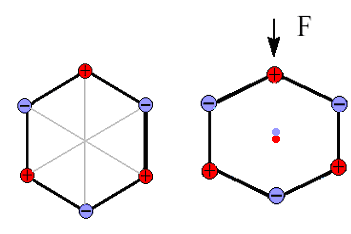
\includegraphics[scale = 1]{1piezo.png}
		\centering
		\caption{Schematische Darstellung des Piezoelektrischen Effekts}
		\label{diagramm_aufspaltung}
	\end{figure}
	Anschaulich lässt sich dies an Figure 3 nachvollziehen. Grundvoraussetzung ist eine symmetrische Verteilung unterschiedlich geladener Ionen im Festkörper, deren Ladungsschwerpunkte sich überlagern, wodurch, im nicht verformten Zustand, kein elektrisches Feld zustande kommt. Für ein piezoelektrisches Element wird der inverse piezoelektrische Effekt benutzt. Dieser besagt, dass auch das anlegen einer Spannung zur mechanischen Verformung eines infrage kommenden Festkörpers führt. Somit wird die angelegte Piezospannung, für das Piezoelement in Z-Richtung, über den Regelkreis so korrigiert, dass der Tunnelstrom konstant gehalten wird. Ziel unserer Rastertunnelmikroskopie ist es, einen vorher festgelegten (X,Y) Bereich "abzurastern" um Informationen über die Elektronenzustandsdichte der Fläche zu bekommen. Um diese Bewegung im nm-Bereich zu gewährleisten, wird der Messkopf in (X,Y)-Richtung auch über ein Piezoelement manövriert. Möchte man die entstehende Realbildaufnahme untersuchen, muss man sich zunächst mit der Struktur der zu untersuchenden, Graphitprobe beschäftigen.
	Graphit ist neben Diamant und Fulleren die dritte unter irdischen Normalbedingungen stabile Form des Kohlenstoffes und kristallisiert meist im hexagonalen Kristallsystem.Es gehört der Mineralklasse "Elemente - Halbmetalle, Nichtmetalle" an. 
	\begin{figure}[h]
		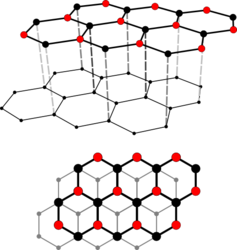
\includegraphics[scale = 1.1]{Graphit.png}
		\centering
		\caption{Aufbau des Graphits}
		\label{diagramm_aufspaltung}
	\end{figure}
	Wie in Figure 4 zu erkennen, besteht der ausgedehnte Kristall aus gestapelten Basalschichten A und B, die so angeordnet sind, dass jeweils drei Kohlenstoffatome einer hexagonalen Zelle über drei Kohlenstoffatomen der darunterliegenden Schicht sitzen. Dies wirkt sich auf die Realbildaufnahme mit dem Rastertunnelmikroskop aus, da ein Kohlenstoffatom der Basalschicht B, welches senkrecht unter einem Atom der Schicht A liegt, dessen elektronische Struktur so beeinflusst, dass die gemessene Elektronenzustandsdichte wesentlich geringer ist, als bei den in Figure 4 rot markierten Kohlenstoffatomen. Dies führt dazu, das wir in der Aufnahme der atomaren Struktur eben diese Atome sehen, wodurch der Eindruck eines größeren Abstandes zwischen den angeordneten Atomen entstehen kann. Eine weitere wichtige Eigenschaft des Graphits ist es, dass die Bindungsenergie innerhalb einer Schicht deutlich größer ist, als die Bindungsenergie zwischen den Schichten (4.3eV zu 0.07eV). Dies führt dazu, dass es leichter ist eine Schicht vom Kristall zu lösen, als einzelne Atome aus einer Schicht. Deswegen ist es uns möglich, Stufenkanten und Plateaus am Graphit zu untersuchen, da diese größtenteils erhalten bleiben. Des Weiteren führt dies zu einer fast metallischen Leitfähigkeit entlang einer Ebene. Wichtige Kenngrößen sind außerdem der Abstand zwischen zwei Kohlenstoffatomen in einer Schicht und der Abstand zwischen zwei übereinander liegenden Kohlenstoffatomen:
	$$a = 2.46 \AA$$
	$$c = 6.71 \AA$$
	Um weitere Informationen und Schlussfolgerungen aus den ermittelten Bildern zu ziehen, unterzieht man die aufgenommenen Topographien einer zweidimensionalen Fouriertransformation. Dabei werden die Bilder vom Real in den Impulsraum, den sogenannten reziproken Raum, abgebildet, wodurch periodische Strukturen besser zu erkennen sind. Durch Rücktransformation lassen sich Störungen der periodischen Struktur extrahieren und man bekommt eine schärfere Abbildung im Realraum.
	
	
	\section{	Versuchsaufbau}
	
	Das in unserem Versuch verwendete Raster-Tunnelmikroskop ist ein Eigenbau der Arbeitsgruppe und arbeitet unter atmosphärischem Druck. Die Bewegung des Messkopfes in X-Y-Z-Richtung wird über einen PC mit der Freeware WSxM der Firma Nanotec gesteuert.  Der schematische Aufbau lässt sich anhand von Figure 5 nachvollziehen.  Die Z-Richtung des Messkopfes wird über einen Regelkreis variiert, um den Tunnelstrom konstant zu halten. Die Bewegung des (X,Y)-Piezo wird über einen Scangenerator gesteuert. Die ankommenden Signale werden verstärkt und an den Messkopf und Spitze weitergeleitet um diese zu bewegen.  Dieser Messkopf besteht im Wesentlichen aus einem Piezo-Röhren-Scanner und einer Messspitze aus einer Titan-Iridium Legierung. Der gemessene Tunnelstrom wird durch einen Strom- / Spannungswandler geschickt, um die gemessenen Ströme (1nA) als Spannung im mV-Bereich besser auswerten zu können. Anschließend werden die Daten logarithmiert um einen größeren Messumfang ohne Bereichsumschaltung zu erreichen. Das Ausgangssignal wird dann an die Bilderzeugung und an den Regler weitergeleitet und der Kreislauf beginnt von neuem. Der gesamte Versuchsaufbau wurde auf einem schwingungsgedämpften Tisch installiert, um Messfehler durch Vibrationen zu minimieren. Des Weiteren befindet sich über dem Versuchsaufbau eine Schutzglocke, um den Messaufbau vor Luftströmen und weiteren Verunreinigungen zu bewahren.
	
	\begin{figure}[h]
		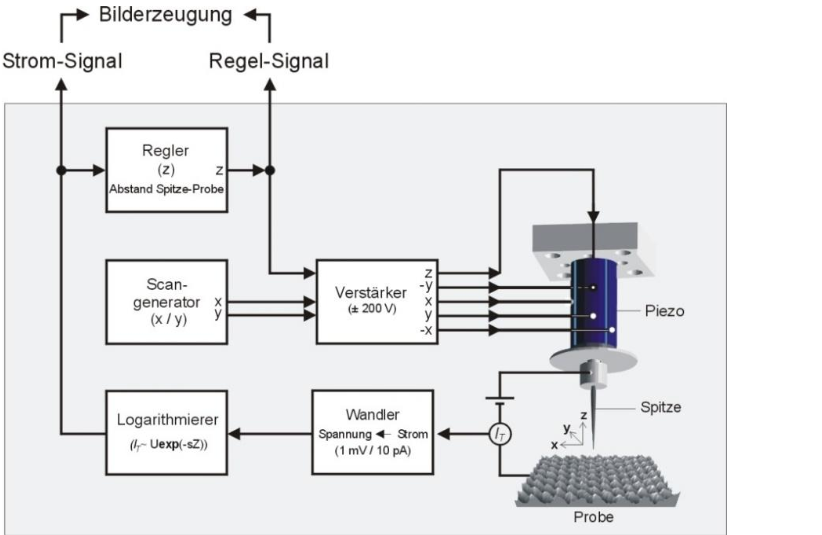
\includegraphics[scale = 0.6]{aufbau.png}
		\centering
		\caption{Blockschaltbild eines Rastertunnelmikroskops}
		\label{diagramm_aufspaltung}
	\end{figure}
	
	\section{Durchführung}
	
	Bevor Messungen am Versuchsaufbau durchgeführt werden können, müssen Messspitze und Graphitoberfläche präpariert werden. Dafür wurde die alte Messspitze zunächst aus dem Aufbau entfernt und mit einer Zange so abgekniffen, dass eine möglichst dünne Spitze erzeugt wurde. Des Weiteren wurde mit einer Lage Tesafilm die oberste Schicht der Graphitprobe entfernt, um mögliche Verunreinigungen zu entfernen und Stufenkanten, bzw. Plateaus zu generieren. Anschließend haben wir die Spitze wieder in den Messkopf eingesetzt und mittels einer Mikrometerschraube per Hand an die Probe angenähert. Mit Hilfe eines Schrittmotors wurde die Spitze dann bis auf wenige $\AA$ angenähert, bis ein vorher festgelegter Tunnelstrom messbar war. Danach wurde der Motor abgenommen und die Schutzglocke aufgesetzt. Anschließend haben wir verschiedene Messungen mit Variationen der Parameter, wie z.B. der angelegten Bias Spannung (zwischen Probe und Spitze) oder des festgelegten Tunnelstroms durchgeführt, um möglichst gute Aufnahmen der Graphit-Oberfläche zu bekommen. Atomare Auflösung konnten wir dabei allerdings nicht erreichen.
	
	\subsection{Parameter}
	
	Zunächst wurde der Messaufbau, wie in der Durchführung beschrieben hergerichtet. Wichtige Parameter sind Size, Speed, Bias, Set Point, Z Gain und der Logarithmic Feedback. Size bestimmt die Kantenlänge der untersuchten Probenoberfläche in nm und der Parameter Speed gibt die Scangeschwindigkeit einer Linie in s an. Bias beschreibt die angelegte Probenspannung in mV und Set Point charakterisiert den konstanten Tunnelstrom während der Messung. Der Z-Gain ist die eingestellte Hochspannungsverstärkung für die Z-Bewegung. Die Funktion des Logarithmic Feedbacks besteht darin, den Fehler zwischen dem gewünschten Sollwert und den gemessenen Werten zu berechnen. 
	
	$$u(t) = K_{p}e(t)+K_{i}  \int_{0}^{t}e(\tau)d\tau$$
	
	Der proportionale Term (mit dem proportional gain $K_{p}$) erzeugt einen Ausgangswert, der proportional zum Fehlerwert $e(t)$ ist und der Integral Term (mit dem integral gain $K_{i}$) summiert die momentanen Fehler über einen Zeitbereich t. Ein kleiner Proportional Gain führt bei einem kleinen Ausgabewert zu einem großen Eingangsfehler.  Sind Proportional und Integral Gain zu hoch, wird der Fehler nicht stabil und beginnt zu oszillieren. In Table 1 haben wir unsere verwendeten Parameter aufgelistet.
	
	\begin{table}[]
		\centering
		\caption{Messparameter}
		\label{Messparameter}
		\begin{tabular}{ll}
			Size (nm)           & 3-30      \\
			Speed (lines / sec) & 1.831     \\
			Points              & 256       \\
			Bias (mV)           & 1000      \\
			Set Point (nA)      & 1-30      \\
			Signal Gain         & 1         \\
			Z Gain              & 1         \\
			Proportional Gain   & 0.2 - 1.8 \\
			Integral gain       & 0.1 - 0.9
		\end{tabular}
	\end{table}

\section{Vermessung von Graphit }

\subsection{ Kantenhöhen}

Mit dem Rastertunnelmikroskop haben wir 79 Bilder aufgenommen. Davon waren 16 zum Kantenvermessen geeignet.
Diese Bilder haben wir mit dem Tool WSxM 4.0 Beta 8.2 vermessen. 
Wir benutzen die Funktionen "Local plane" und "profile". "Local plane" reskaliert, nach Auswahl von ebenen Flächen, das gesamte Bild.  Die Funktion "profile" liefert ein Höhenprofil der Verbindungslinie zwischen zwei ausgewählten Punkten (Siehe Bilder der Kanten unten).
Viele Bilder waren fehlerhaft und konnten nicht zur Bestimmung von Kantenhöhen verwendet werden.
Ursachen dafür waren thermische Verschiebung (Drift), Creep, Bildfehler \ref{b12} oder keine verwertbare Kanten auf den Bildern. Wir haben jede Kante an 5 unterschiedlichen Orten vermessen, dies lieferte den Mittelwert und den Fehler als Standardabweichung.



\subsection{Beispiel Kanten}

\begin{figure}[]
	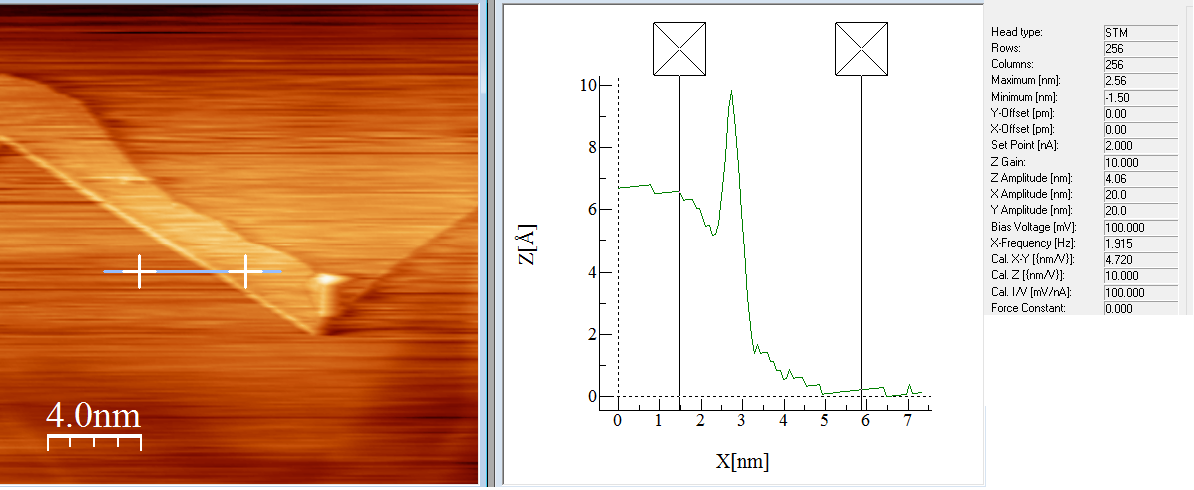
\includegraphics[scale = 0.3]{bild00.png}
	\centering
	\caption{Bild 0. Kante 0.637 nm und RTM Daten}
	\label{b0}
\end{figure}

\begin{figure}[]
	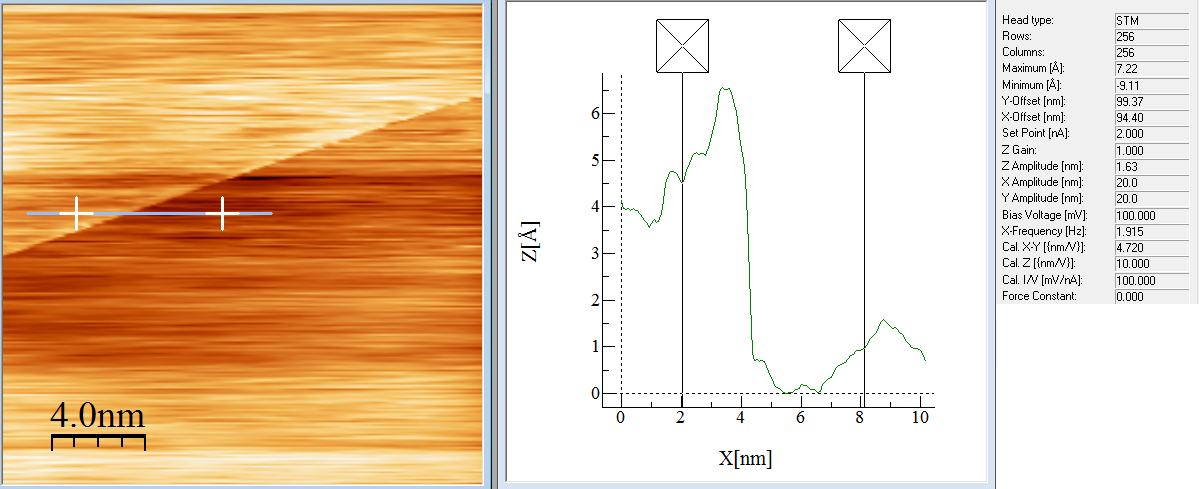
\includegraphics[scale = 0.3]{bild11.png}
	\centering
	\caption{Bild 11. Kante 0.353 nm und RTM Daten}
	\label{b11}
\end{figure}
\begin{figure}[]
	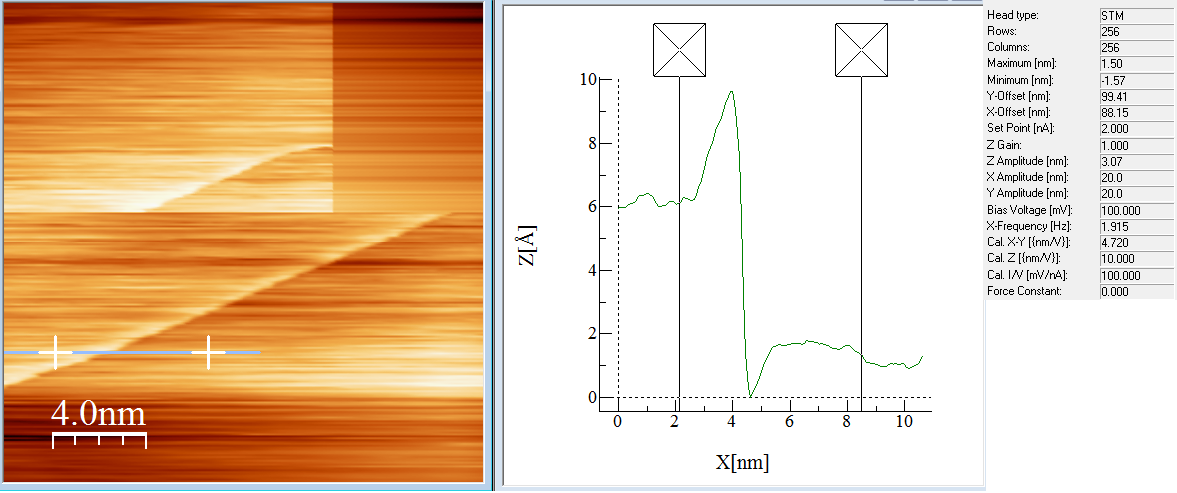
\includegraphics[scale = 0.3]{bild12.png}
	\centering
	\caption{Bild 12. Kante 0.447 nm und RTM Daten}
	\label{b12}
\end{figure}




In dem Diagramm \ref{kantendia} sind alle gemittelten Kanten eingetragen. Die Höhen gingen von 0.272  $ \pm 0.149 $ nm bis 1.893 $ \pm 0.250 $ nm. Die theoretischen Kanten wurden mit den roten Linien markiert.

\begin{figure}[]
	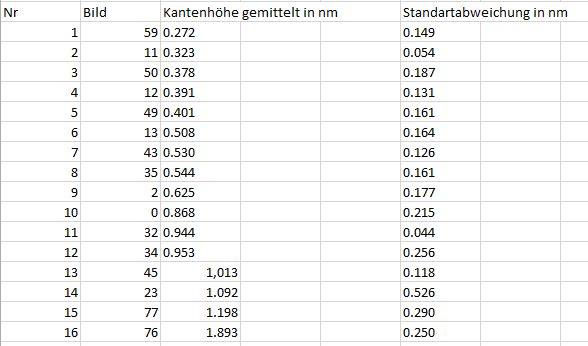
\includegraphics[scale = 0.5]{Kantengeordnetrichtig.png}
	\centering
	\caption{Liste der geordeneten Kanten}
	\label{list}
\end{figure}

\begin{figure}[]
	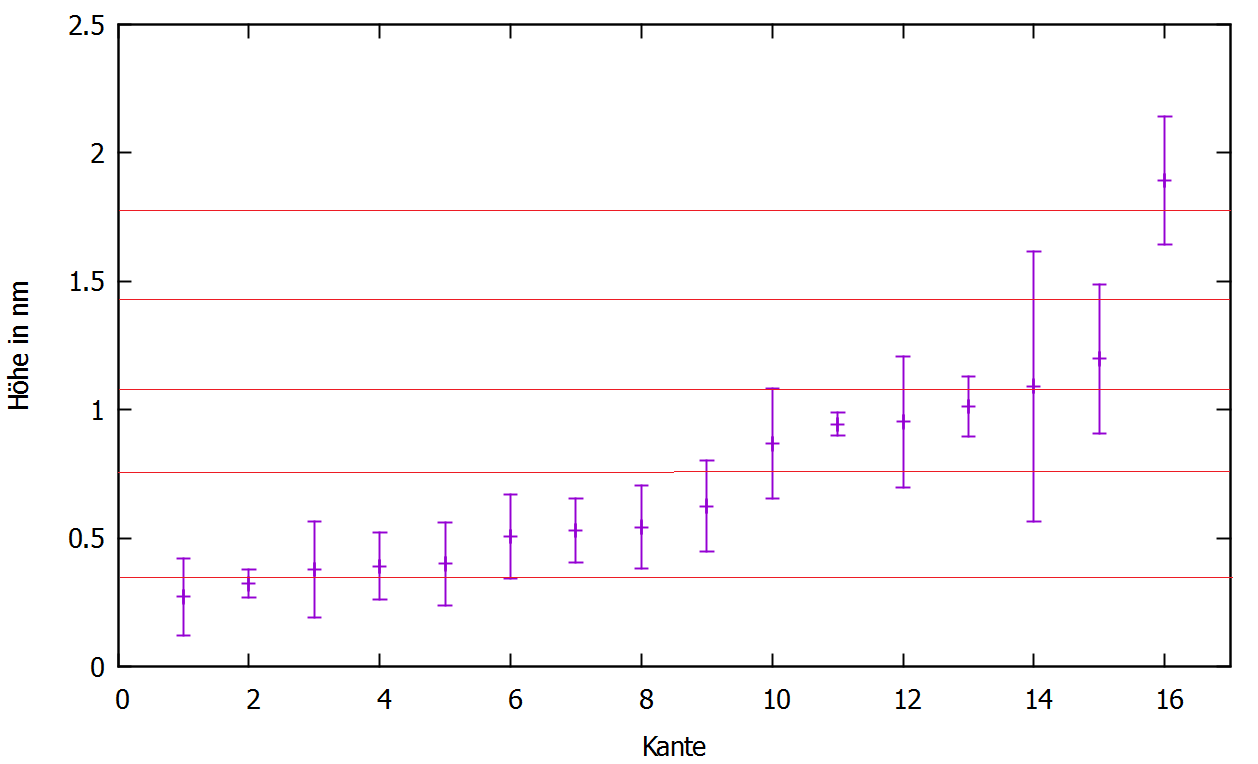
\includegraphics[scale = 0.5]{kantendiag.png}
	\centering
	\caption{Diagramm Höhe der Kanten sowie in Rot die theoretische Kantenhöhen}
	\label{kantendia}
\end{figure}

In dem Diagramm\ref{kantendia} sehen wir eine Ansammlung von Messwerten bei der erst- und dritten Kante. Diese Kanten werden deshalb am besten durch unsere Messungen repräsentiert. Die anderen theoretischen Kanten werden nur bedingt durch unsere Messergebnisse widergespiegelt.
Anhand des Graphen ordnen wir die ersten sechs Kanten der einfachen Gitterkonstante zu, da die Fehlerbalken über den theoretische Ebenenabstand geht. Kante 7 und 8 sind genau zwischen zwei theoretischen Kanten und danach wird die Zuordnung von Kante zu n-fachen der Gitterkonstante nicht einfacher.
Jede Kante wurde der n- fachen Ebenenabstand zugeordnet, dessen Mittelpunkt am nächsten der theoretischen Ebene war. Kante 7 und 8 wurden daher ausgelassen, da eine eindeutige Zuordnung nicht möglich war(genau zwischen zwei Gitterkonstanten). Unsere gemessene Gitterkonstante ist $(3.5 \pm 0.6) \mathring{A}$. Werte entstehen aus dem Mittelwert der durch n gewichteten Kanten und dessen Standardabweichung. \\ 
q =  $\frac {theo. Ebenenkosntante} {gemessene Ebenenkonstante}$\\
Der q- Wert ist wichtig für die Kalibrierung des Z - Piezos.
Gehen wir nun von der Kalibrierung des Z- Piezos mit 10 nm per Volt aus, müssen wir diesen Wert auf $10 \frac {nm} {v} * q = (9.5 \pm1.5)nm$ nach unten korrigieren.


\subsection{Ebene Grafitoberfläche}

Zum Untersuchen der atomaren Struktur von Grafit, haben wir versucht eine ebene Fläche in unserer Probe zu finden und sie zu messen. Die Feinheit der zur Messung verwendeten Sensorspitze ist ausschlaggebend dafür, wie exakt Strukturen auf der Grafitoberfläche gemessen werden können. Weil wir die Spitze mit einer Zange, durch das abkneifen eines Drahtes, hergestellt haben, war die Wahrscheinlichkeit groß, dass der Sensor zum Messen der atomaren Struktur nicht fein genug ist. Obwohl wir ebene Flächen im Grafit fanden, war es nicht möglich atomare Strukturen zu erkennen.

Deshalb haben wir zur Untersuchung der atomaren Struktur die Daten aus den Referenzmessungen verwendet. Die Messung aus den Referenzmaterialien kann in Abbildung \ref{Grafitoberflächenebene} gesehen werden. Hier ist \ref{grafob1} die rohe Messung an sich. Es ist die ebene Oberfläche des Grafits zu erkennen. In \ref{grafob2} haben wir mithilfe einer doppelten Fouriertransformation Störungen aus der Messung entfernt. Dadurch lässt sich die atomare Struktur genauer untersuchen.

\begin{figure}[h]
	\centering
	\begin{subfigure}{0.45\textwidth}
		\centering
		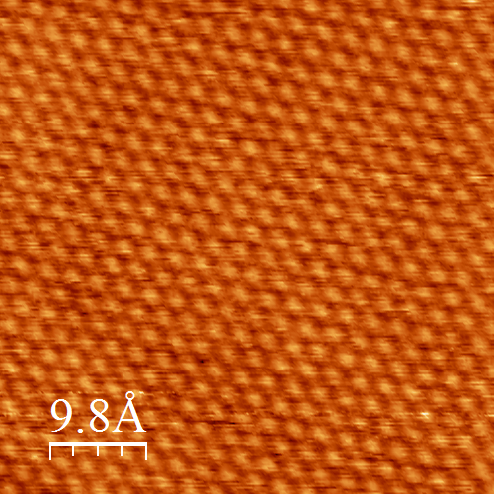
\includegraphics[width=\textwidth]{vor_doppelter_fourier.png}
		\caption{gemessene Grafitoberfläche}
		\label{grafob1}
	\end{subfigure}
	\begin{subfigure}{0.45\textwidth}
		\centering
		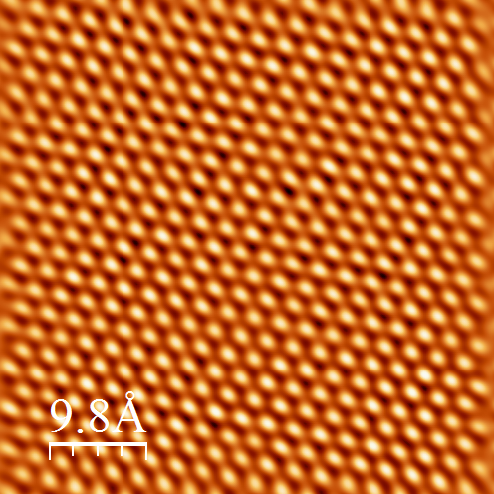
\includegraphics[width=\textwidth]{nach_doppelter_fourier.png}
		\caption{Gemessene Grafitoberfläche, nachdem Störungen durch eine doppelte Fouriertransformation beseitigt wurden}
		\label{grafob2}
	\end{subfigure}
	
	\caption{Messung des Tunnelstroms an einer ebenen Fläche Grafit}
	\label{Grafitoberflächenebene}
\end{figure}

Es kann klar erkannt werden, dass die Kohlenstoffatome regelmäßig in einer Kristallstruktur angeordnet sind. Man erkennt ein hexagonales Kristallsystem, wie es für Grafit zu erwarten war.

\begin{figure}[h]
	\centering
	
	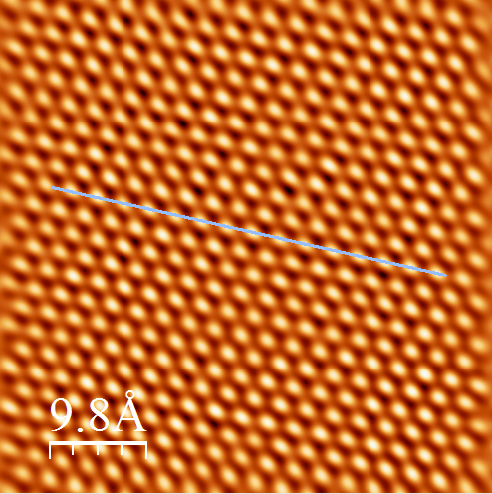
\includegraphics[scale = 0.4]{Aufnahme_Ebene_doppelte_fourier2.png}
	
	\caption{Messung der Abstände der atomaren Erhebungen}
	\label{Messungerh1}
\end{figure}

\subsubsection{Messungen an atomaren Erhebungen} \label{kapitolo}

Entlang der in \ref{Messungerh1} zu sehenden Geraden haben wir die Abstände der atomaren Erhebungen gemessen. Das zu Gerade 1 dazugehörige Diagramm kann in Abbildung \ref{Messungerh2} gesehen werden. Wir haben alle Abstände entlang der zu sehenden Geraden gemessen und anschließend Mittelwerte mit Standardabweichungen gebildet. Die gemessenen Abstände für alle atomaren Ausrichtungen sind in Tabelle \ref{Messungerh5} zu sehen. Unsere Werte für den Abstand der atomaren Erhebungen ist entlang Gerade 1 $(0,265 \pm 0,002) nm$, Gerade 2 $(0,273 \pm 0,002) nm$ und Gerade 3 $(0,222 \pm 0,003) nm$. Unsere durch die Standardabweichung erhaltenen Fehler von $0,002 nm$ beziehungsweise $0,003 nm$, sind kleiner, als es physikalisch sinnvoll wäre. Alleine der Fehler durch die Schwingung des Gitters, abhängig von der Temperatur sollte größer sein. Deshalb nehmen wir für unsere Fehler den Standardfehler der Messwerte. Damit sind unsere Werte für die Abstände der atomaren Erhebungen $(0,27 \pm 0,01) nm$, $(0,27 \pm 0,01) nm$ und $(0,22 \pm 0,01) nm$

Laut der Theorie sehen wir in dem mit dem Rastertunnelmikroskop aufgenommenen Bild nur jedes zweite Atom des Grafit-Kristalls. Der planare Abstand nächster Nachbarn im Kristall ist mit $b = 0,142 nm$ gegeben. Der von uns zu erwartende Abstand der atomaren Erhebungen lässt sich mithilfe des Kosinussatzes als 

\begin{equation}
	s = b \cdot \sqrt{2(1-cos(120^\circ))} = 0,246 nm
	\label{eq:aabstand}
\end{equation}

berechnen. Die Rechnung kann anhand von Abbildung \ref{rechnungatomabstand}, in der die hexagonale Struktur Grafits dargestellt ist, hergeleitet werden. Unsere Werte stimmen mit dem dritten Fehlerintervall mit dem theoretischen Wert überein. Hätten wir die Standardabweichung als Fehler genommen, würden unsere Werte über 10 Fehlerintervalle von dem theoretischen abweichen.

\begin{figure}[h]
	\centering
	
	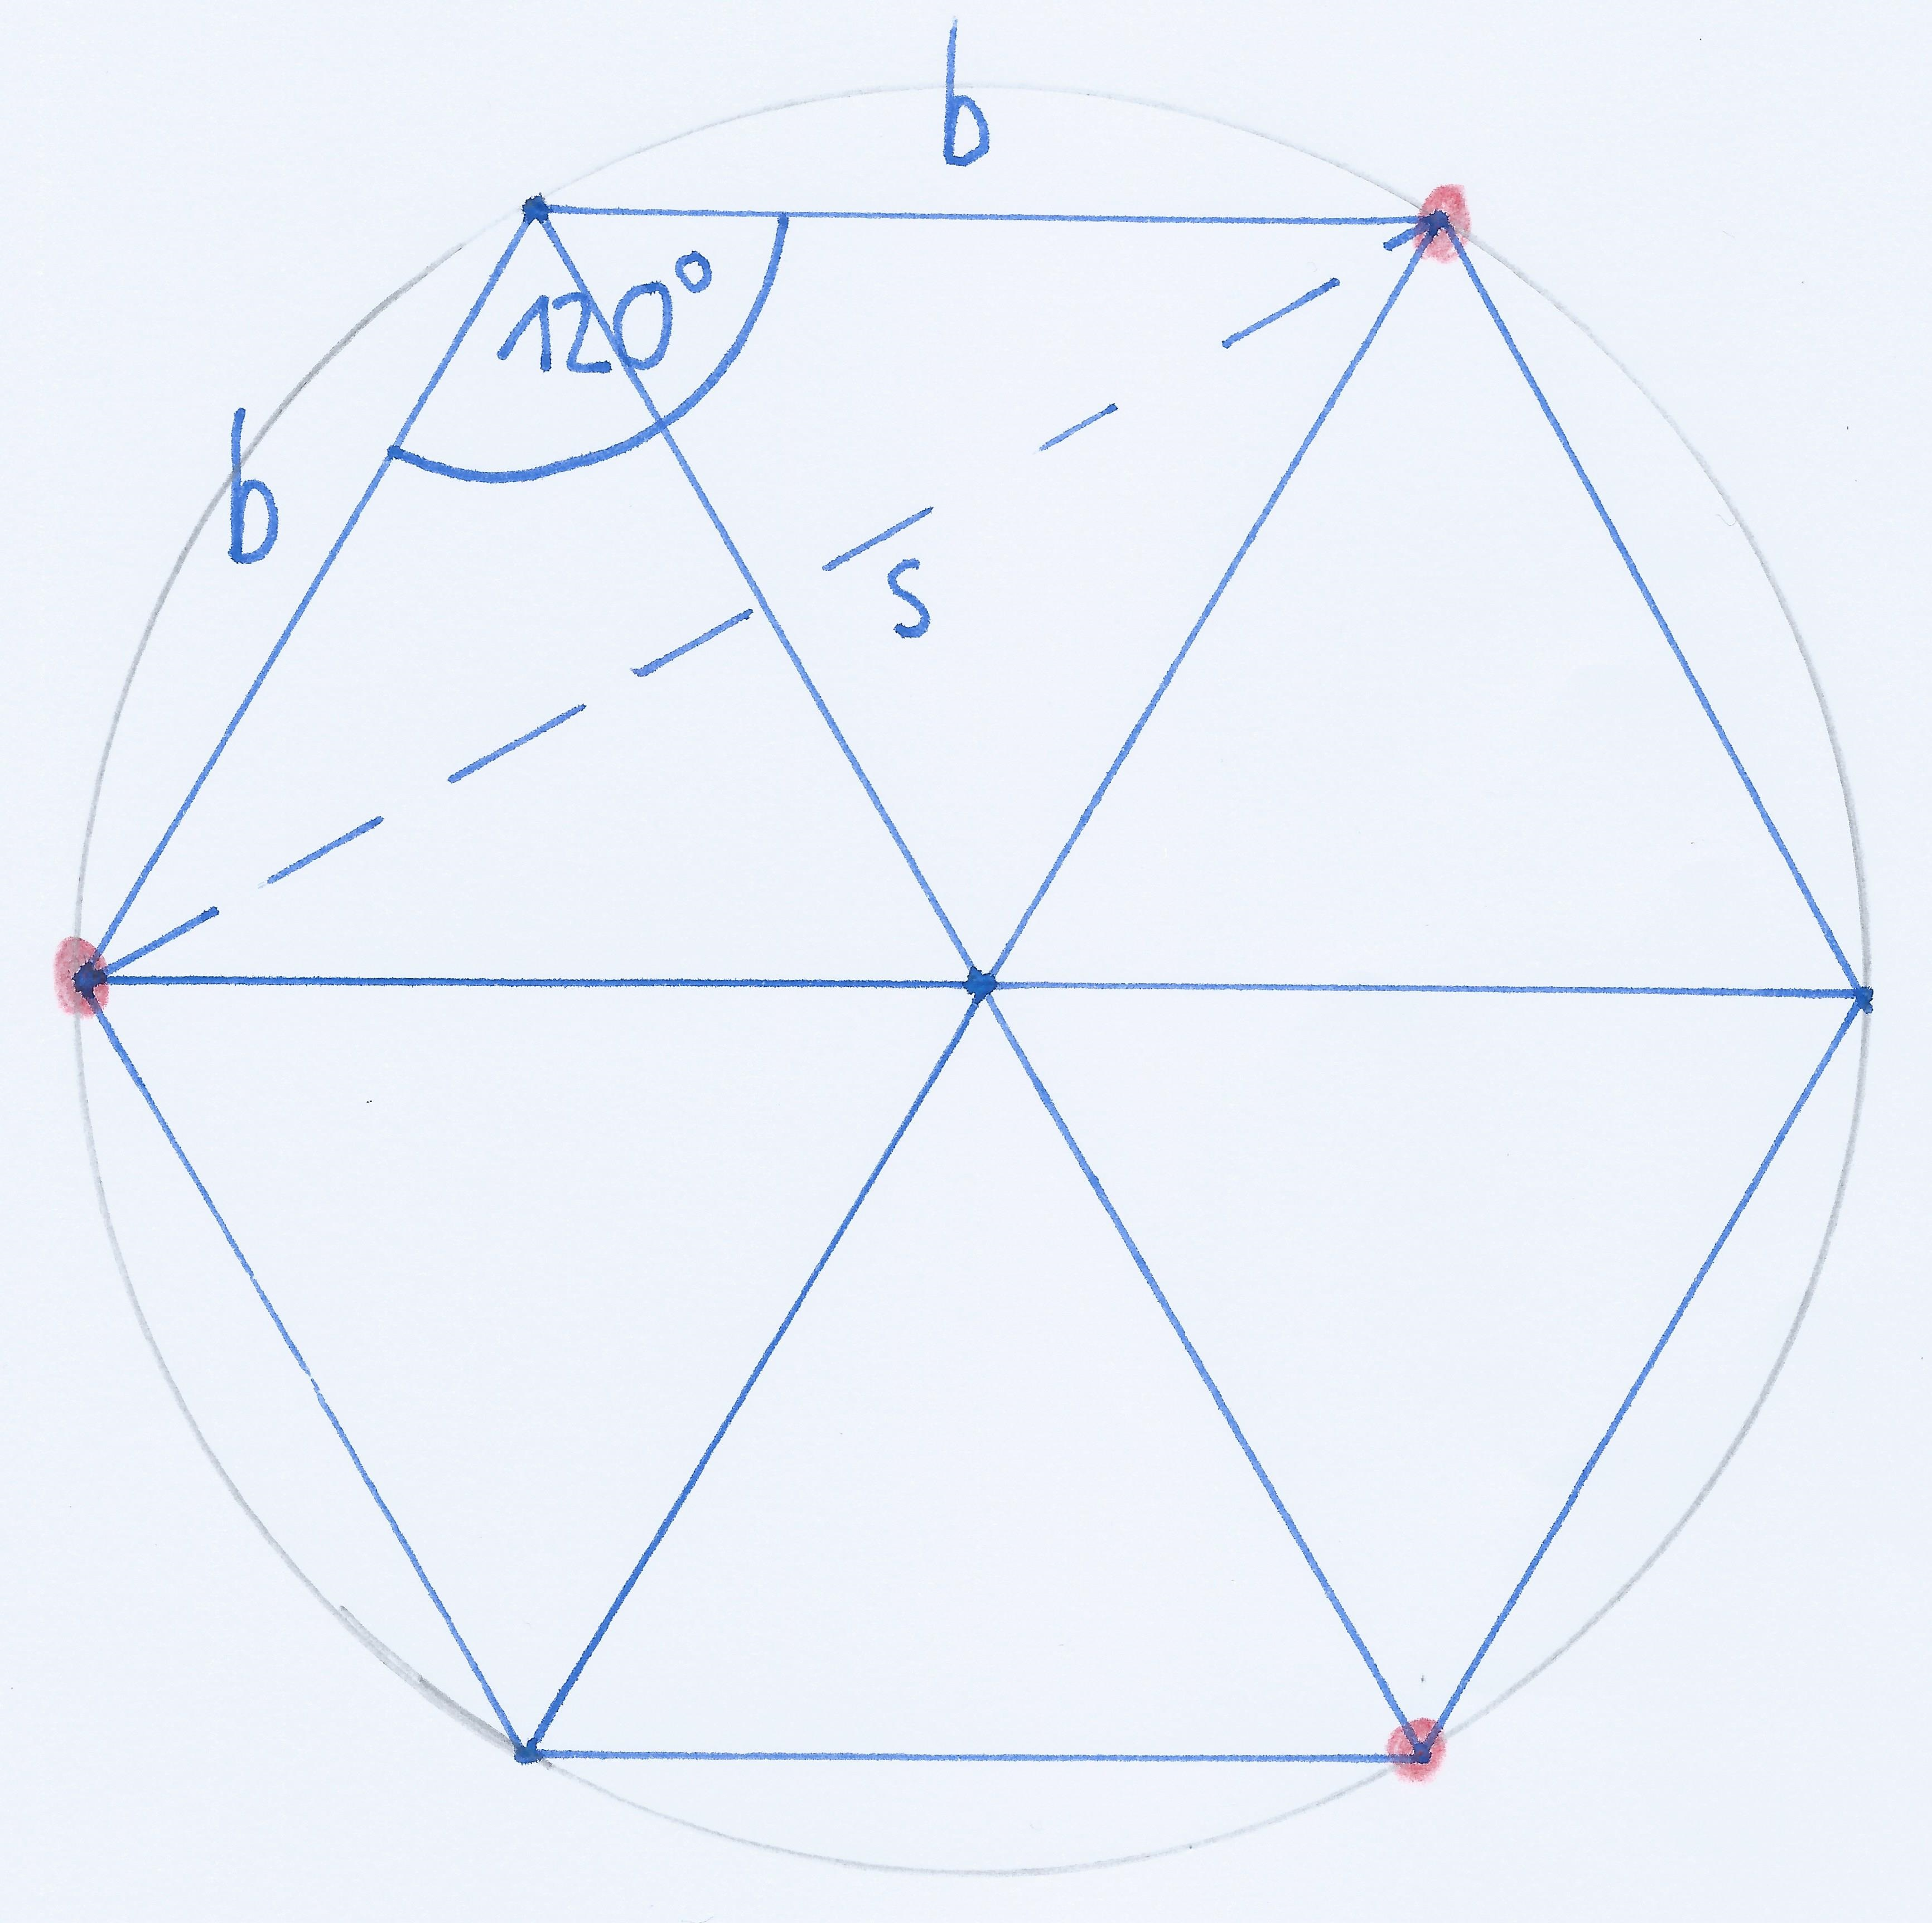
\includegraphics[scale = 0.4]{hexagon.jpg}
	
	\caption{Hexagonale Struktur des Grafits: Im Rastertunnelmikroskop sichtbare Atome sind rot gekennzeichnet}
	\label{rechnungatomabstand}
\end{figure}

Eine wichtige Größe, die großen Einfluss auf den Messfehler hat, ist die Temperatur während der Messung. Sie beeinflusst die Energie des Kristalls und somit auch seine Eigenbewegung. Eine weitere Fehlerquelle, dass unser Wert nicht mit dem theoretischen übereinstimmt wäre, dass wir mit dem Rastertunnelmikroskop nicht senkrecht zur Probe messen. Dieser Fehler ist jedoch so klein einzuschätzen, dass er nicht ausschlaggebend für die vom theoretischen Wert abweichenden Messwerte ist. Eine größere Fehlerquelle ist, dass der Sensor in einem Raster über die Ebene fährt. Dies tut er mit Hilfe von einem X- und Y-Piezoelement. Sind die Piezoelemente nicht richtig kalibriert, so kommt es in den Messbildern zu Verzerrungen. Diese Verzerrungen stellen einen systematischen Fehler dar, der erklären würde, weshalb alle von uns gemessenen Werte entlang einer atomaren Ausrichtung über beziehungsweise unter dem theoretischen Wert liegen (mehr zur Verzerrung durch die Piezoelemente in Kapitel \ref{winkelsec}). Daraus folgt, dass unser gemessener Wert möglicherweise mit dem theoretischen übereinstimmen könnte, wenn man den systematischen Fehler entfernen würde.  

Eine weitere Fehlerquelle, die eine Verzerrung des Messbildes verursachen könnte, ist eine Temperaturdifferenz zwischen Messspitze und Probe. Durch eine solche Temperaturdifferenz, würde die Messspitze mit der Probe durch Wärmetransport wechselwirken und somit das Messbild beeinflussen. Je länger der Sensor über einer Stelle der Probe sitzt, desto mehr Wärme wird zwischen Sensor und Probe ausgetauscht. Deshalb ist dieser Fehler besonders klein, wenn sich der Sensor schnell über die Probe bewegt. Zur Aufnahme unserer Messbilder bewegt sich der Sensor in einem Raster über die Probe. Weil er sich dabei die meiste Zeit in der horizontalen Achse der Messbilder bewegt, sollte die durch die Temperaturdifferenz auftretende Verzerrung in diese Richtung am geringsten sein. In unseren Messaufnahmen sollten deshalb, wenn der sogenannte thermische Drift der dominante Fehler ist, die atomaren Abstände entlang Gerade 1 am meisten den theoretischen entsprechen. Dies ist nicht der Fall. Unsere gemessenen Messwerte weichen entlang aller atomaren Ausrichtungen gleich weit von dem theoretischen Wert ab.

Wenn die Piezoelemente die Ursache der Verzerrung sind, könnte man diese durch eine Neukalibrierung der Elemente beheben. Eine weitere Methode wäre es, den systematischen Fehler der Verzerrung numerisch zu lösen. Es könnte auch versucht werden, durch eine Änderung der Geschwindigkeit, mit der der Sensor über die Probe fährt, der Verzerrung entgegenzuwirken.

\begin{figure}[h]
	\centering
	
	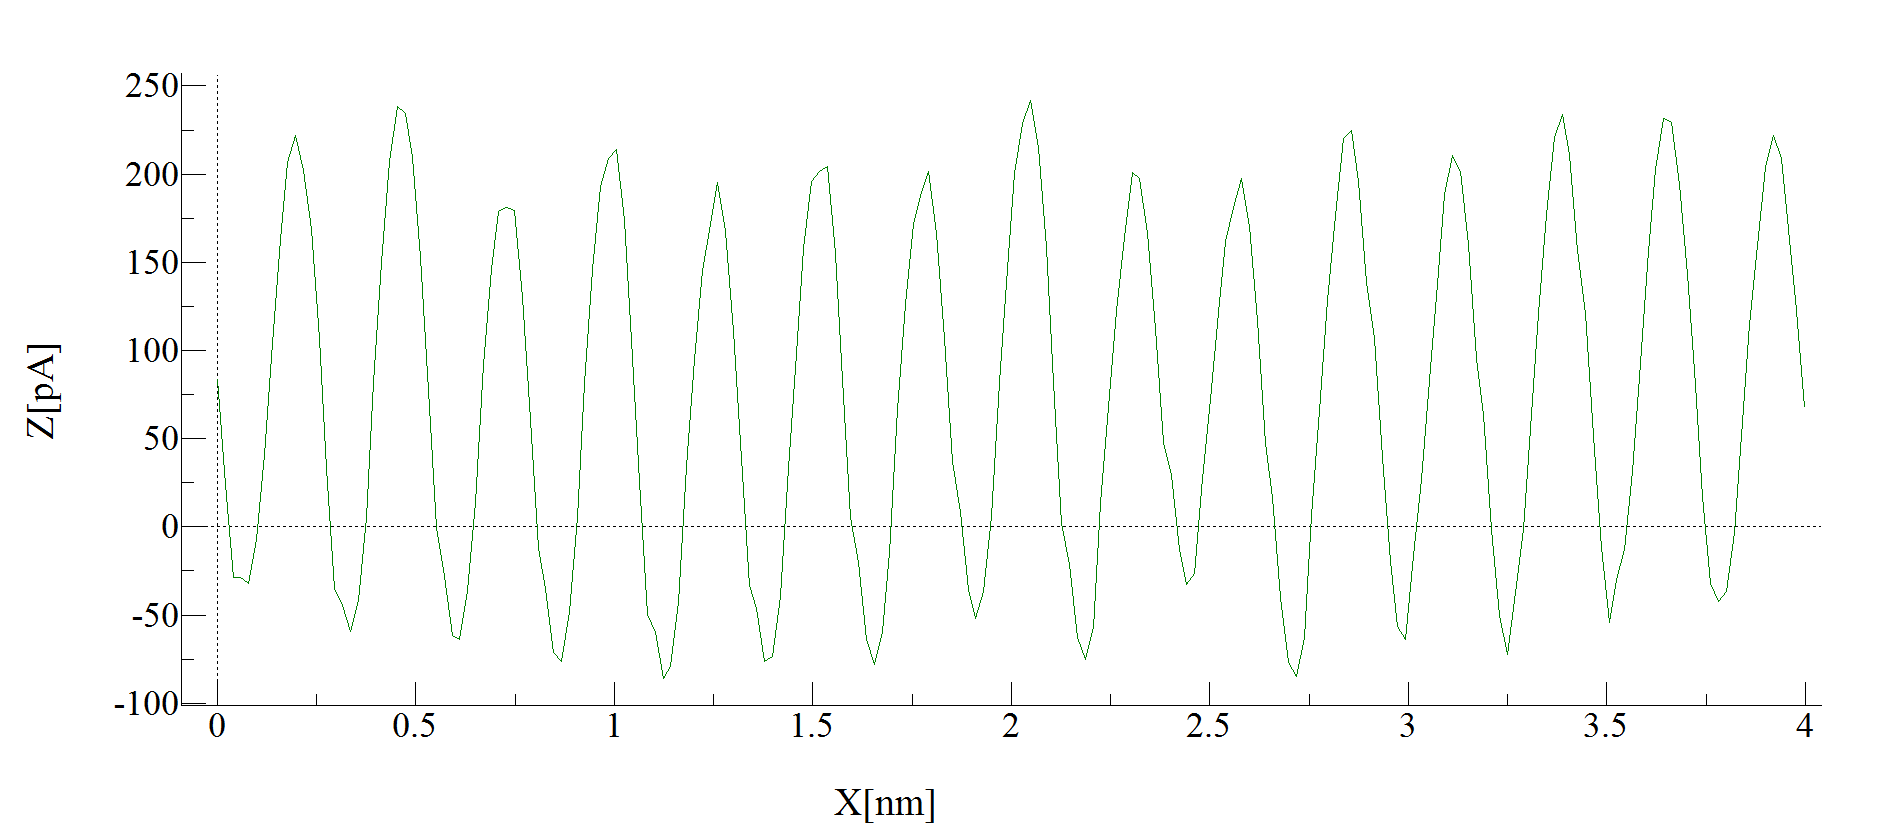
\includegraphics[scale = 0.3]{Aufnahme_Ebene_doppelte_fourier.png}
	
	\caption{Diagramm zur Messung der Abstände der atomaren Erhebungen}
	\label{Messungerh2}
\end{figure}

Zur Messung der Höhe der atomaren Erhebungen wurden die Messdaten, welche die Höhen und nicht den Tunnelstrom angeben, verwendet. Auf diesen Messdaten waren die atomaren Erhebungen selbst nach einer doppelten Fouriertransformation sehr ungenau zu erkennen, wie in Abbildung \ref{Messungerh3} zu sehen ist. Im Vergleich zu Abb. \ref{grafob2} sind die atomaren Erhebungen unschärfer und Erhebungen, die sich horizontal anordnen sind weniger abgegrenzt, als welche, die sich vertikal anordnen. Dies kommt wahrscheinlich dadurch zustande, dass der Sensor in einem Raster über die Probe fährt.

Wir haben entlang der in Abbildung \ref{Messungerh3} zu sehenden Geraden gemessen. Das zu der Geraden gehörende Diagramm kann in Abb. \ref{Messungerh4} gesehen werden. An diesem Diagramm haben wir durch das Bilden der Differenz von Maxima und Minima die Höhen der atomaren Erhebungen gemessen. Die Werte können in Tabelle \ref{Messungerh5} gesehen werden. Nach dem Bilden eines Mittelwerts und einer Standardabweichung erhält man für den Wert der Höhe $(8,8 \pm 0,4) pm$.

Der theoretische Wert für den Abstand benachbarter Ebenen in Grafit ist $335 pm$. Dieser Wert übersteigt die von uns gemessene Höhe der atomaren Erhebungen um zwei Größenordnungen. Folglich lassen sich unsere gemessenen Höhen nicht mit diesem Wert identifizieren. Um nachzuvollziehen, wie unsere gemessenen Höhen der atomaren Erhebungen zustande kommen, müssen wir die Form der Metallspitze, die wir als Sensor benutzen, mit in Betracht ziehen. In diesem Fall betrachten wir eine einatomige Sensorspitze. Das führende Atom der Spitze hat einen gewissen Durchmesser und kann, wenn sein äußerstes Orbital ein s-Orbital ist, als eine Kugel mit gewissem Radius verstanden werden. Lässt der Tunnelstrom zwischen Sensor und Probe nach, fährt dieser näher an die Probe heran. Dies ist zum Beispiel zwischen den atomaren Erhebungen der Fall. Weil die Metallspitze jedoch einen Radius hat, wird sie, wenn sie über einer Stelle zwischen den atomaren Erhebungen ist, mit diesen beim Versuch sich der Probe anzunähern "zusammenstoßen" (Orbitale von Spitze und Probe überlappen sich). Deshalb sind die gemessenen Höhen der atomaren Erhebungen viel kleiner als der tatsächliche Ebenenabstand.

\begin{figure}[h]
	\centering
	
	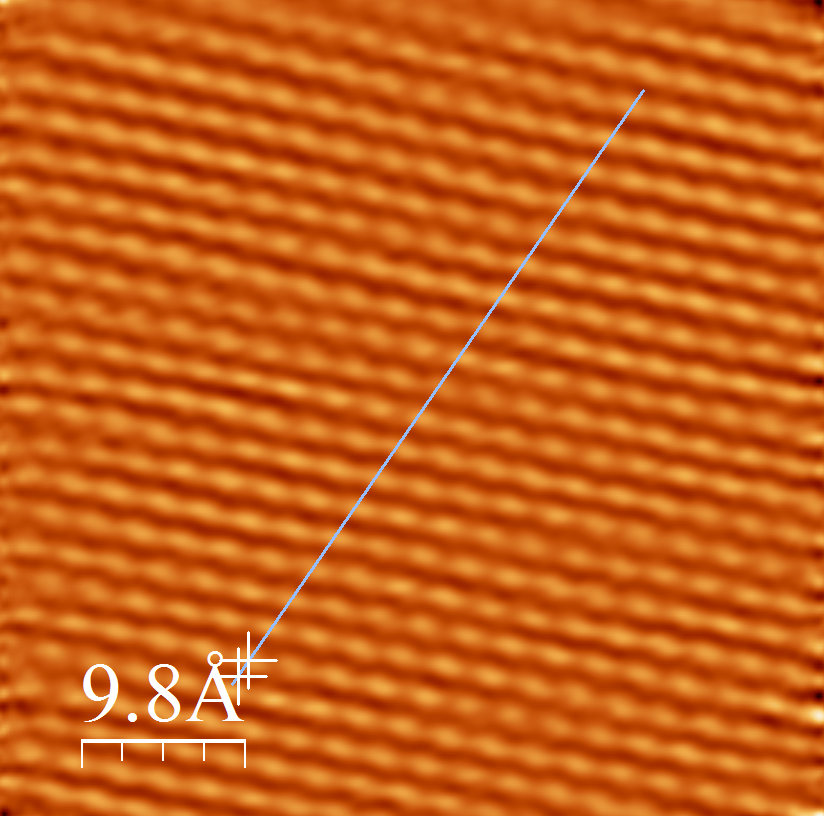
\includegraphics[scale = 0.4]{hohenmessung11.png}
	
	\caption{Messung der Höhe der atomaren Erhebungen}
	\label{Messungerh3}
\end{figure}

\begin{figure}[h]
	\centering
	
	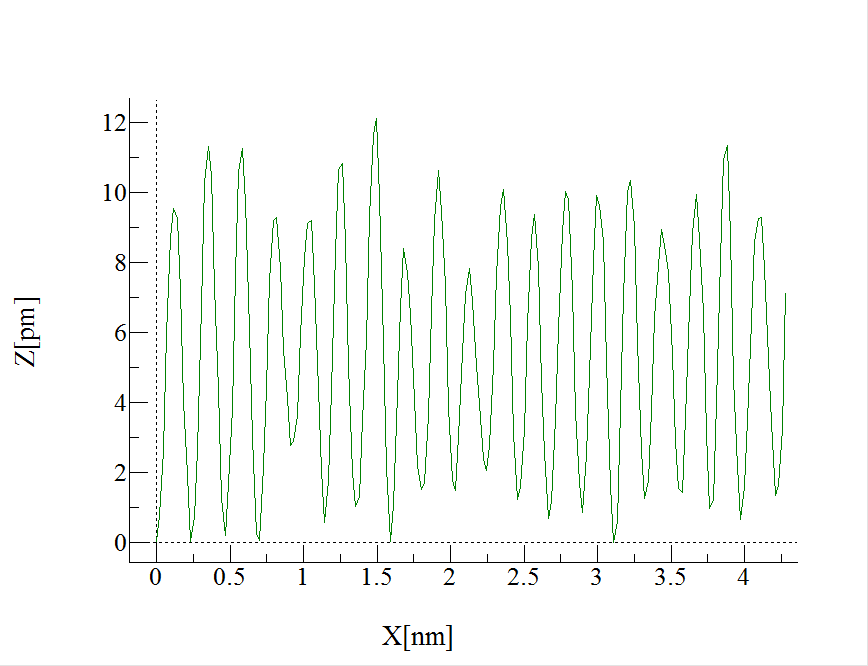
\includegraphics[scale = 0.7]{hohenmessung1_diagramm.png}
	
	\caption{Diagramm zur Messung der Höhe der atomaren Erhebungen}
	\label{Messungerh4}
\end{figure}

\begin{table}[h!]
	\centering
	\begin{tabular}{|l|l|l|l|}\hline
		Abstand & Abstand & Abstand & Höhe/pm $\pm 0,3 pm$\\
		Ausrichtung 1/nm $\pm 0,01 nm$ & Ausrichtung 2/nm $\pm 0,01 nm$ & Ausrichtung 3/nm $\pm 0,01 nm$ & \\\hline
		0,26 & 0,28 & 0,21 & 9,4 \\
		0,27 & 0,28 & 0,23 & 10,9 \\
		0,26 & 0,28 & 0,22 & 11,0\\
		0,26& 0,28 & 0,24 & 6,4 \\
		0,26 & 0,28 & 0,21 & 8,4 \\
		0,27 & 0,27 & 0,22 & 9,7 \\
		0,26 & 0,28 & 0,23 & 11,9\\
		0,27 & 0,26 & 0,20 & 6,7\\
		0,26 & 0,26 & 0,24 & 9,0\\
		0,27 & 0,27 & 0,21 & 5,7\\
		0,26 & 0,27 & 0,24 & 8,7\\
		0,28 & 0,28 & 0,21 & 8,5\\
		0,26 & 0,27 & 0,23 & 8,8\\
		0,27 &  & 0,20 & 9,6\\
		&  & 0,23 & 8,8\\
		&  & 0,24 & 7,4\\
		&  & 0,22 & 8,7\\
		&  & 0,24 & 10,2\\
		&  &  & 7,8\\
		\hline
	\end{tabular}
	\caption{Gemessene Werte für die Abstände und Höhen der atomaren Erhebungen entlang verschiedener atomarer Ausrichtungen}
	\label{Messungerh5}
\end{table}

\subsubsection{Winkel und Symmetrien} \label{winkelsec}

Anhand von Abbildung \ref{Messungerh6} haben wir die Winkel zwischen den atomaren Richtungen gemessen. Unsere gemessenen Winkel, startend von dem Winkel rechts oben und dann entgegen dem Uhrzeigersinn laufend, sind $63^\circ$, $67^\circ$, $48^\circ$, $67^\circ$, $66^\circ$ und $49^\circ$, mit jeweils einem Fehler von $1^\circ$. Wegen der hexagonalen Struktur von Grafit wäre bei einer naiven Herangehensweise zu erwarten, dass alle Winkel $60^\circ$ sind. Dies ist nicht der Fall. Es fällt auf dass die besonders kleinen Winkel($48^\circ$ und $49^\circ$) entgegengesetzt voneinander liegen. 

Die Winkel sollten nicht alle bei $60^\circ$ sein, wenn man mit dem Sensor nicht senkrecht zur Probe misst. Damit Winkel von $60^\circ$ auf $48^\circ$ heruntergehen, müsste man jedoch mit viel größeren Winkeln zum Lot auf die Probe gucken, als es bei unserem Experiment der Fall ist. Dass die Winkel von $60^\circ$ abweichen muss also eine andere Erklärung haben.

Eine wahrscheinlichere Erklärung für die unterschiedlichen Winkel ist, dass wegen der die Probe im Raster abfahrenden Sensorspitze, das Messbild verzerrt wird. Der Sensor wird mithilfe von Piezoelementen entlang der X- und Y-Achse verschoben. Es kann sein, dass das Piezoelement, das für die Verschiebung in X- oder Y-Richtung verantwortlich ist, nicht richtig kalibriert ist. In diesem Fall fährt der Sensor nicht über die Fläche, die in den Messdaten angegeben ist. Ist zum Beispiel das Piezoelement für die y-Richtung falsch kalibriert, kann es sein, dass es eine größere Strecke abfährt, als es sollte. Weil das Programm zum Berechnen der Messbilder eine andere Strecke erwartet, wird das Messbild in y-Richtung gestaucht. Dadurch verändern sich die gemessenen Abstände und Winkel von den tatsächlichen. Durch diesen Messfehler lassen sich die bei uns von $60^\circ$ abweichenden Winkel erklären. Auch erklärt dieser Fehler, wieso die kleinsten Winkel entgegengesetzt voneinander sind.

Der schon in Kapitel \ref{kapitolo} erklärte thermische Drift könnte ebenfalls eine Verzerrung der Messbilder und damit unterschiedliche Winkel zwischen den jeweiligen atomaren Ausrichtungen erklären.

Die von uns beobachteten atomaren Erhebungen des Grafits bilden ein hexagonales Kristallgitter. Es ist 6-zählig. Entlang einer Translation von ganzzahligen Abständen der atomaren Erhebungen der in \ref{Messungerh6} eingezeichneten Linien, gibt es außerdem eine Translationssymmetrie. Zusätzlich sieht man, dass bei einer Spiegelung entlang einer der Geraden und einer Inversion an dem Punkt, in dem sich die Geraden schneiden, das Gitter symmetrisch ist.

\begin{figure}[h]
	\centering
	
	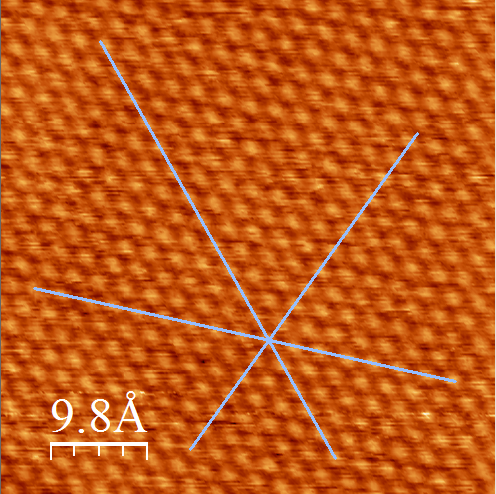
\includegraphics[scale = 0.7]{Winkelmessung_kristall.png}
	
	\caption{Messung der Winkel zwischen den atomaren Richtungen}
	\label{Messungerh6}
\end{figure}

\subsection{Fouriertransformation einer ebenen Fläche Grafits}

In Abbildung \ref{fouriertansformation_ebene} kann das Gitter aus Abbildung \ref{grafob1} nach einer Fouriertransformation betrachtet werden. Man erkennt sechs Punkte, die auf einem leicht verzerrten Hexagon um den Ursprung liegen. Um den Ursprung herum sieht man Werte in geringer Intensität. Dies sind die Störungen, die beim Aufnehmen der Messung entstanden sind. Die sechs zu erkennenden Punkte beinhalten alle Informationen über die Periodizität des gemessenen Gitters. Jedem der sechs Punkte kann ein Vektor $\vec{k}$ zugeordnet werden. Dies ist ein Wellenvektor, der eine Periodizität des Gitters angibt. Verschiebt man das Gitter also um eine Periode der Welle, die mit dem Wellenvektor $\vec{k}$ zu assoziieren ist, bleibt das Gitter unverändert. Daraus lässt sich leicht folgern, dass man aus $\vec{k}$ mit der folgenden Gleichung direkt den Abstand zweier atomarer Erhebungen berechnen kann.

\begin{equation}
	|k| = \frac{2\pi}{a}
	\label{formelk}
\end{equation}

Hier ist a der Abstand zweier atomarer Erhebungen.

Die aus Abb. \ref{fouriertansformation_ebene} mit \eqref{formelk} berechneten Werte für die Abstände der atomaren Erhebungen sind $(2,1\pm0,1)\mathring{A}$, $(2,0\pm0,1)\mathring{A}$ und $(2,5\pm0,1)\mathring{A}$. Wir haben drei Werte, weil von den sechs k-Werten jeweils zwei zu einer Periodizität gehören. Weil der Abstand der atomaren Erhebungen entlang aller atomaren Ausrichtungen gleich groß sein sollte, wäre auch zu erwarten, dass alle in der Fourierdarstellung gemessenen k-Werte gleich groß sind. Wegen der Verzerrung der Messbilder, sind die k-Werte jedoch unterschiedlich. Der dadurch entstehende Fehler für die Berechnung der atomaren Abstände in größer, als der direkte Messfehler einer atomaren Ausrichtung aus dem Messbild. 
Nur einer der drei Messwerte stimmt mit kleiner gleich drei Fehlerintervallen mit dem theoretischen Wert von $2,46\mathring{A}$ überein.
Um gute Messwerte für die atomaren Abstände zu erhalten, müsste man die Verzerrung der Messbilder entfernen.

%Deshalb geben wir den mithilfe der k-Vektoren berechneten Wert der Abstände der atomaren Erhebungen als Durchschnittswert mit der Standardabweichung als Fehler an. Der berechnete Wert ist $(2,2 \pm 0,3)\mathring{A}$. Er stimmt mit den in \eqref{eq:aabstand} theoretisch berechneten Wert von $2,46\mathring{A}$ überein. Es scheint, dass sich wegen der Verzerrung der Messbilder, die Fourierdarstellung des Gitters weitaus besser zum Bestimmen das Abstands der atomaren Abstände eignet, als das direkte Ausmessen in den Messbildern.

\begin{figure}[h]
	\centering
	
	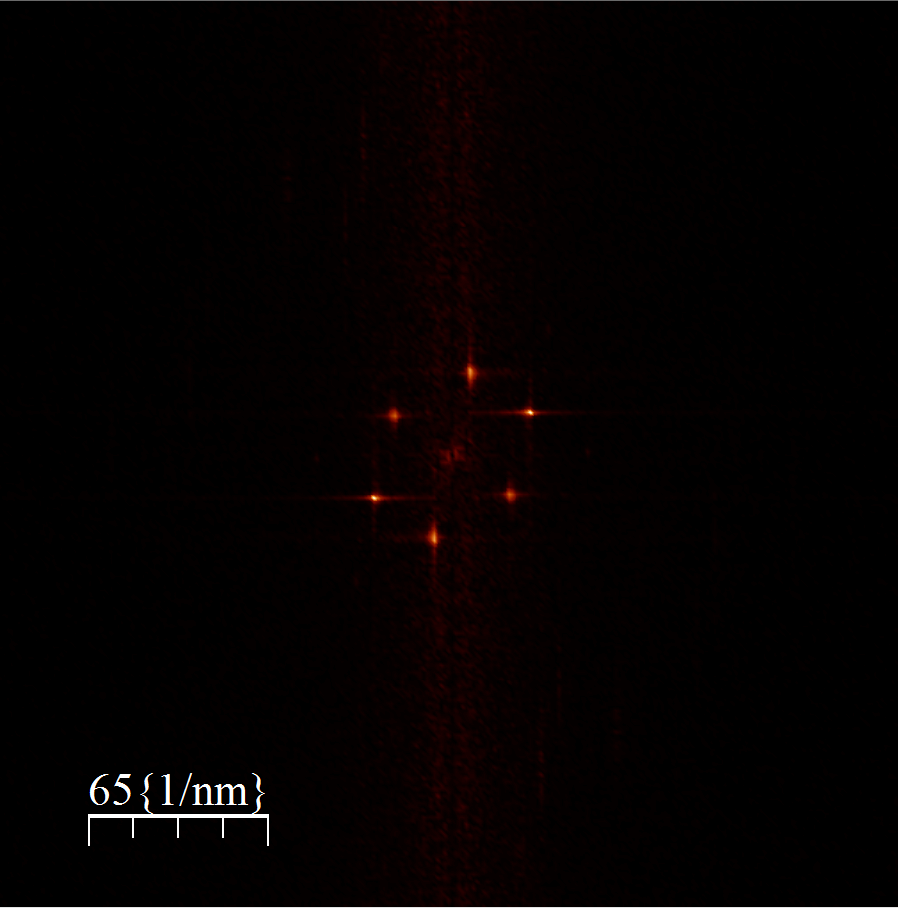
\includegraphics[scale = 0.5]{Fouriertrasformation_kristall.png}
	
	\caption{Fouriertransformation von Abbildung \ref{grafob1}}
	\label{fouriertansformation_ebene}
\end{figure}

\section{ Diskussion}

Beim Vergleichen der theoretischen Kanten mit dem Messergebissen muss drauf geachtet werden, dass die Kanten nicht durch Drift oder Creep unscharf werden, bzw. keine Kanten im Kristall sind. Die Form der Spitze ist entscheidend. Da diese mit einer Drahtschere gefertigt wurde(keine einatomige Spitze), sind größere Messfehler zu erwarten. Weitere Fehlerquellen sind die Ungenauigkeit und Inhomogenität des Piezos und die Graphitprobe selbst.
Mit unseren Messbildern konnten wir 16 Kanten an der Graphitoberfläche vermessen. Diese Kanten wurden nach der Höhe geordnet und in Diagramm \ref{kantendia} dargestellt. Wir konnten mit unseren Messergebnissen, wegen den großen Fehlerwerten, die theoretischen Kanten relativ schlecht darstellen. Vor allem den ersten und dritten Netzebenenabstand können unsere Messergebnisse rekonstruieren. Einige Messergebisse sind fast genau zwischen zwei Ebenen, dies könnte an der schlechten Wahl von Messpunkten in Messbildern liegen. Eine Vorsondierung der Bilder wäre von Nöten gewesen, um mehr Kanten zu erfassen und die Ergebnisse klarer zu gestalten.
Der von uns, mit dem Kantenhöhen bestimmte Ebenenabstand des Graphits ist $(3.53 0.58)\mathring{A}$ und damit im einfachen Fehlerintervall zum Literaturwert von 3.35 $\mathring{A}$, was dem großen Fehler unserer Messdaten zugrunde liegt. (Quelle: Anleitung zum Rastertunnelmikroskop, BA10 Fu Berlin Praktikum)
\\\\
Nach dem Vermessen von Kanten, haben wir die Kristallstruktur Grafits näher betrachtet. Da unsere Sensorspitze nicht fein genug war, konnten wir zwar Kanten an der Oberfläche, die atomare Struktur des Grafits jedoch nicht erkennen, beziehungsweise nur eingeschränkt über eine kleine Fläche. Deshalb mussten wir zur Betrachtung der Struktur von Grafit Referenzmessungen benutzen.

Anhand der Referenzdaten untersuchten wir die hexagonale Struktur des Grafits. Es konnten Translations-, Inversions-, Spiegelungs- und Rotationssymmetrien erkannt werden. Die leicht unterschiedlichen Größen der Winkel zwischen den atomaren Richtungen konnten wir damit erklären, dass das X- oder Y-Piezoelement zum Bewegen des Sensors nicht richtig kalibriert war.

Unsere aus den Messbildern abgelesenen Werte für die Abstände der atomaren Erhebungen waren entlang der verschiedenen atomaren Ausrichtungen $(2,7 \pm 0,1) \mathring{A}$, $(2,7 \pm 0,1) \mathring{A}$ und $(2,2 \pm 0,1) \mathring{A}$. Sie wichen mit 3 Fehlerintervallen von dem theoretischen Wert von $2,46 \mathring{A}$ ab. Es erwies sich, dass sich die Abstände mithilfe einer Fouriertransformation besser bestimmen ließen. Die aus der Fouriertransformation bestimmten Werte waren $(2,1\pm0,1)\mathring{A}$, $(2,0\pm0,1)\mathring{A}$ und $(2,5\pm0,1)\mathring{A}$. Einer der Werte stimmt mit dem theoretischen überein, während die anderen Werte über 3 Fehlerintervalle von ihm abweichen.
Auch wenn die Werte aus der Fouriertransformation nur zum Teil bessere Ergebnisse, als die aus den Messbildern liefern, ist ihr Fehler besser einzuschätzen. Die Verzerrung der Messbilder kann sofort bei Betrachtung der Fourierdarstellung erkannt werden. Bei einer direkten Betrachtung der Messbilder war die Verzerrung erst nach dem Ausmessen der Winkel zwischen den atomaren Ausrichtungen oder dem Berechnen der Abstände der atomaren Erhebungen zu erkennen.

Bei einer richtigen Kalibrierung des X- und Y-Piezoelements könnte man eine Verzerrung der periodischen Strukturen des Gitters möglicherweise verhindern. Dadurch könnte man die Messung der atomaren Abstände anhand der Fourierdarstellung präziser und mit kleinerem Messfehler durchführen. Eine numerische Lösung der Verzerrung wäre möglich, jedoch mit hohem Aufwand verbunden.
Es ist nicht auszuschließen, dass die Verzerrung der Messbilder nicht durch falsch kalibrierte Piezoelemente, sondern durch den thermischen Drift zustande kommt.

Um bessere Versuchsergebnisse zu erzielen, könnte man die Sensorspitze des Rastertunnelmikroskops mit einer anderen Methode herstellen. Die Feinheit der Sensorspitze ist für den Erfolg des Versuchs ausschlaggebend und bestimmt, ob es möglich sein wird, die atomare Struktur des Grafits zu messen.




\section{Quellen}
(Figure 1):\url{https://elearning.physik.uni-frankfurt.de/data/FB13-PhysikOnline/lm_data/lm_282/auto/kap26/picts/tunnel.gif}\\
(Figure 2):\url{http://www.uni-ulm.de/physchem-praktikum/media/fp/v_11.pdf}\\
(Figure 3):\url{http://www.piezoeffekt.de/bilder/1piezo.gif}\\
(Figure 4): \url{https://upload.wikimedia.org/wikipedia/commons/thumb/5/54/GraphitGitter4.png/237px-GraphitGitter4.png}\\
(Figure 5): Blockschaltbild eines Raster-Tunnelmikroskops von Frank Trixler, Ludwig-Maximilians-Universität München (Aus der Anleitung)
\end{document}